\documentclass{article}
\usepackage{amsmath}
\usepackage{amssymb}
\usepackage{amsthm}
\usepackage{graphicx}
\usepackage{caption}
\usepackage{subcaption}
\usepackage{float}
\usepackage{subfig}
\usepackage{hhline}
\usepackage{multirow}
\usepackage{supertabular}
\usepackage{color}

\theoremstyle{plain}% 
\newtheorem{thm}{Theorem}[section]
\newtheorem{lem}[thm]{Lemma}
\newtheorem{prop}[thm]{Proposition}
\newtheorem{cor}[thm]{Corollary}

\theoremstyle{definition}
\newtheorem{defn}{Definition}[section]
\newtheorem{rem}{Remark}[section]


\title{Non-linear Least Squares Problem \\{\Large Final Project in  Numerical Optimization}}
\date{}
\author{Bastian Haase}

\begin{document}
\maketitle
\tableofcontents
\newpage 
\section{Introduction}
Non-linear least squares problems form an important subcategory of numerical
optimization. One of their most important applications lies in data fitting, which is, for instance, an important tool in statistics. A typical nonlinear least squares problem has the form 
$
  f(x)=\frac{1}{2}\sum_{i=1}^{m} r_j^2(x)
$
for smooth functions $r_j: \mathbb{R}^n\rightarrow \mathbb{R}$, which are called  \emph{residuals}. Let $r=(r_j)_{j=1,..,m}^T$ denote the \emph{residual vector} and $J$ its Jacobian. A short
computation shows 
\begin{align*}
  \nabla f(x)= J(x)^Tr(x)\; \textrm{ and } \; \nabla^2 f(x)= J(x)^TJ(x)+ \sum_{i=1}^m r_j(x)\nabla^2 r_j(x),
\end{align*}
which reveals an interesting feature of these problems: By computing the Jacobian $J$, one already
gets the first term of the Hessian of $f$. Often, the residuals are small or nearly linear, in these cases the term $J^TJ$ is a good approximation of the Hessian that can be used in Newton's method. This method is called Gauss-Newton and performs very well in a wide range of problems. However, one frequently occurs problems with large residuals at the initial guess and/or at the solution where  the described approximation
might not yield satisfying results. In this work, I want to describe algorithms that also approximate the
second term and analyze how well these algorithms perform in the large residual case. 
\subsection{Aim of this Work}
The aim is to implement and compare 3 different strategies to approximate $S(x)=\sum_{i=1}^{m}r_i(x) \nabla^2f(x)$ in a Newton method. We will test them against standard implementations
of the Newton method, Gauss-Newton and BFGS. The first strategy relies on approximating $\nabla^2 f(x)$ by finite differences and to use this to approximate $S(x)$. Furthermore, we will implement two strategies proposed by Brown-Dennis (\cite{Brown1971}) and
Dennis-Gay-Welsh (\cite{Dennis1981}) which approximate and update the term $S(x)$. It should be noted
that Dennis-Gay-Welsh propose their update strategy in combination with a very sophisticated 
trust-region algorithm. This algorithm does not just adjust the trust region but also
decides between their new update strategy or a standard Gauss-Newton model. As this work
focuses on the approximation of $S(x)$, I will not implement the trust-region algorithm. 
Note that such an algorithm could also be paired with any other update strategy tested here. Finally,
we will implement an algorithm proposed by Fletcher-Xu (\cite{Fletcher1987}). It is a hybrid
algorithm of Gauss-Newton and BFGS using line-search. This method chooses between Gauss-Newton and BFGS steps between
each iteration depending on a parameter which we will tweak for every test problem.
\section{Test Problems}
In this section, we will briefly describe the test problems and their characteristics.
All problems chosen are theoretical problems designed to test non-linear least squares problems
(cmp. \cite{Brown1971}), so they suit this project. For all test problems, our termination
criterion will be a gradient norm less than $10^{-8}$.
\subsection{Freudenstein's Problem}
Freudenstein's problem is given by the equation 
\begin{align*}
   f(x)=\frac{1}{2}((x_1-13+((5-x_2)x_2-2)x_2)^2+(x_1-29+((x_2+1)x_2-14)x_2)^2)
\end{align*}
which has dimensions $m=n=2$. It has a global minimum at {\color{red}$(5.0,4.0)$} with a residual of zero and 
a local minimum at approximately {\color{green}$(11.4128,-0.8968)$} where the residual is roughly $24.4921$.
Our initial guess is {\color{blue}$x_0=(6.0,6.0)$} with a residual of $12025$. The colors indicate their position in
Figure \ref{surface}.
\subsubsection{Characteristics}
This problem has small dimensions and the residuals are linear in one variable and cubic in the
other. Our starting point has a large residual, while the minima have very low residuals.
It will be interesting to see, whether one of the algorithms will converge to the local
minimum with non-zero residual.\par
Figure \ref{surface} shows us that there is a ''bump'' between both minima and that
our starting point is at a point with a very high slop in the $x_2$ direction.
\begin{figure}
    \centering
        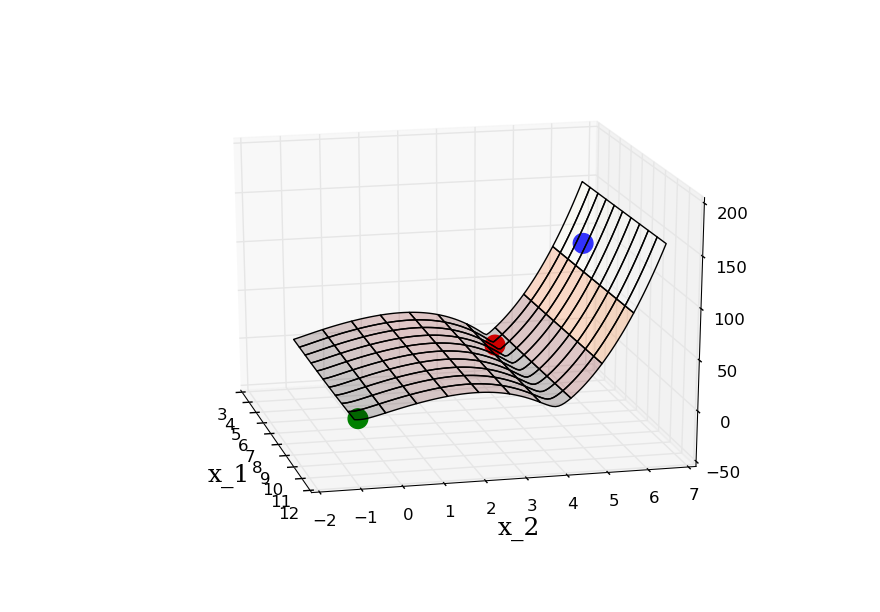
\includegraphics[width=0.8\textwidth]{contour_freudenstein.png}
        \caption{Surface Plot of $\sqrt{\text{Freudenstein}}$}
        \label{surface}
\end{figure}
\subsection{A Classical Problem}
The following problem is a long-known, popular, non-linear least squares problem. It is given by
the function 
\begin{align*}
  f(x)=\frac{1}{2}\sum_{k=1}^{10} \left(e^{-0.1kx_1}-e^{-0.1kx_2}-x_3\left(e^{-0.1k}-e^{k} \right) \right)^2
\end{align*}
which has zero residual whenever $x_1=x_2$ and $x_3=0$. There is an additional zero
residual at $x=(1,10,1)$. The dimensions of this problem are 
$n=3$ and $m=10$. We will use the starting point $x_0=(0,10,20)$ where the residual
is approximately $1031.154$. 
\subsubsection{Characteristics}
In this problem, the residual at the starting point is large, yet the residual at the minimum
is zero. This suggests that Gauss-Newton should perform very well once we are close enough 
to a solution. We expect that the specialized algorithms should outperform the Gauss-Newton
at the beginning, while it is unclear whether their performance close to a minimum will be
competitive. We will  investigate whether all algorithms will converge to the same solution.
The residuals are linear in one component, yet exponential in the other two components.
\subsection{Nielsen's Problem}
Nielsen's problem is a data-fitting problem.  It is given by the data in Table 1
\begin{table}[H]
  \centering
  \begin{tabular}{|l|c|c|c|c|c|c|c| c|c|c|}
    \hline
   \textbf{j} & 0 & 1 & 2 &3 & 4 & 5 & 6 & 7 & 8 & 9 \\ \hline
  \textbf{y}  & 2.0 & 0.0 & 2/3  &0.0 & 2/5 & 0.0 & 2/7 & 0.0 & 2/9 & 0.0 \\ \hline
  \end{tabular}
  \caption{Data underlying Nielsen's problem}
  \label{tab:dataNielsen}
\end{table}
and the functional relationship 
\begin{align*}
  r_j(x)=x_1x_3^j+x_2x_4^j
\end{align*}
for $j=0,\ldots,9$. So the dimensions of the problem are $n=4$ and $m=10$. 
The minimum is achieved at $(0.97754,0.97754,-0.65140,0.65140)$ with a residual of
$0.03734$. Out inital guesses will be $x_0=(1.0,1.0,-0.75,0.75)$ (\emph{Nielsen1}) where the residual is
also only $0.13484$. and $x_0=(1.0,2.0,-2.0,1.0)$ (\emph{Nielsen2}) with a residual of  $174009.4725$.
\subsubsection{Characteristics}
The Hessian is not linear in any component. It will be interesting
to see how the performance changes from the low residual initial guess to the large
residual inital guess. 
\subsection{Trig Problem}
Consider the problem given by 
\begin{align*}
  f(x)=\frac{1}{2}\sum_{k=1}^{20} \left(\left(x_1-0.2kx_2-e^{0.2k} \right)^2+\left(x_3+x_4\sin(0.2k)-\cos(0.2k)\right)^2 \right )^2
\end{align*}
with dimensions $n=4$ and $m=2$. The minimum is approximately at $x=(-11.594,13.204,-0.40344,0.23678)$ with a residual of approximately $85822$. We will choose the starting point $x_0=(25.0,5.0,-5.0,-1.0)$ where the residual is approximately $7926693$.
\subsubsection{Characteristics}
Note that the residuals are quadratic in every component. This problem has a large residual even
at the solution, which will challenge our algorithms in a  different way than the preceding problems
do. We would expect that the specialized large residual problems outperform the other algorithms
the most here.
\section{The Algorithms}
In this section, we will describe all algorithms that we have tested. Our descriptions will
be more detailled when discussing the problems designed for non-linear least squares problems
with large residual.
\subsection{Standard Algorithms}
We will test our specialized algorithms against a couple of standard algorithms. As we
can actually compute the Hessian matrices for all four problems, we will use a modified
implementation of Newton's method that modifies the Hessian by adding an appropriate multiple of the identity matrix if
Cholesky factorization fails. Newton's method does not converge
globally, but it provides quadratic convergence locally. The method can obviously
not be used when the Hessian is not available and should be avoided when the Hessian is
costly to construct.\par
We will furthermore use a standard implementation of
BFGS that updates an approximation of the inverse of the Hessian. This algorithm is
a standard algorithm that is very popular for problems where the Hessian is unavailable
or costly. But, note that this algorithm is more generic and designed to handle many different types of optimization
problems. It does not take our special setting into account.  We have guaranteed global convergence but can only expect superlinear
convergence, even when being close to the solution.\par
Lastly, we will also test Gauss-Newton. We described this method in the beginning as
the standard algorithm for non-linear least squares problem with a small residual.
It takes the special structure of our problem into consideration and basically
approximates our Hessian for free (given that we compute the gradient anyway),
but this approximation will be inaccurate when the residual is large and 
the residual functions are not linear. Henceforth, we  expect this method to
perform poorly when the residuals are big. This should be very prominent in the trig problem,
while it could be less influential for the other problems where the residual at the solution
is small. 
\subsection{Approximated Newton}
We have implemented Newton's method where we use an approximation of the Hessian
instead of the real Hessian. But, to take our scenario into account, we will not approximate
the whole Hessian vie finite differences, but instead only the hessians of the residuals $
  \nabla^2 r_j(x)$.
We expect that this method performs very similar to Newton's method for all of our
problems, as this behavior was observed in homework 3 in this class. \par
One should note that this method is very costly in terms of gradient evaluations
and might therefore be impractical in problems of high dimensions with complex
gradients. We will subsequently refer to this method as \emph{appNew}.
\subsection{Brown-Dennis}
We describe Algorithm 2.1 in \cite{Brown1971}. The idea is to approximate
$\nabla^2 r_j$ and update the approximation after each iteration. Then, one applies a regular
Newton step. The initial
approximation is chosen to be done by finite differences, i.e. the first step of
the Brown-Dennis method is the same as the approximated Newton method. \par
Subsequently, let $B_{i,k}$ denote the approximation of $\nabla^2 r_i(x_k)$.
Then, the update formula is given by 
\begin{align*}
  B_{i,k+1}=B_{i,k}+\left(\nabla r_i(x_{k+1})^T- \nabla r_i (x_k)^T-B_{i,k}\Delta x_k \right)
\frac{(x_{k+1}-x_k)^T}{\|\Delta x_k \|_2^2}.
\end{align*}
The second summand can be interpreted as follows: Recall that $B_{i,k}$ is an approximation of
$\nabla^2 r_i(x)$. Thus, the term inside the brackets resembles the error of the first Taylor
polynomial of $\nabla r_i(x)$ centered around $x_k$ and evaluated at $x_{k+1}$. Thus, the whole
second term is approximating this error in the direction of the last step. From this point of view,
one also notices the resemblence to BFGS and the SR1 update.\par
Brown-Dennis prove the following theoretical result concerning convergence of this method.

\begin{thm}
  Let $x^*$ be a critical point and let $\Omega$ be a convex neighborhood. Let $K_i\geq 0$ be constants such that for every $x \in \Omega$, we have $\| \nabla^2 r_i(x)- \nabla^2 r_i(x^*)\| \leq K_i \| x- x^*\|$ for $i=1,\ldots, m$. \par
 Then, whenever $\nabla^2 f(x^*)$ is nonsingular, there exist constants $\epsilon,\delta>0$ such that  the algorithm converges for any $x_0 \in \Omega$ with $\|x_0-x^*\|< \epsilon$ and $\|B_{i,0}-\nabla^2 r_i (x_0) \|\leq \delta$. \par
Furthermore, the convergence is at least quadratic when $f(x^*)=0$.
\end{thm} 
\begin{proof}
  Compare Theorem 1 and 2 in \cite{Brown1971}.
\end{proof} 
\begin{rem}
  Brown and Dennis prove more convergence results that do not need the assumption that a solution exists.
However, these results only give superlinear convergence and require assumptions on the 
accuracy of their approximation $B_{ik}$.
\end{rem}
\subsection{Dennis-Gay-Welsh}
In their paper \cite{Dennis1981}, Dennis, Gay and Welsh propose the algorithm \emph{NL2SOL}
that is implemented in many software packages for numerical optimization.  Contrary
to the last update formula, this approach updates an approximation to $S(x)$ instead of approximations to each $\nabla^2 r_i(x)$, so it requires less storage. The approximation is based on
the secant condition. This update is also sized before updating, as this has proven to
yield a more robust algorithm. \par
In their paper, they propose this update formula in combination with a sophisticated algorithm that uses two different update
strategies and a trust region approach. To be more precise, it  uses a quadratic model
on an elliptic trust region and starts with the Gauss-Newton method. Then, during
every iteration, the algorithm decides whether to switch to the other method (Gauss-Newton or
their new update strategy described below) and whether to adjust the trust region. The algorithm
always tries to switch the method before shrinking the trust region. \par
It should be noted that this approach does not depend on the two methods that one has chosen.
One could for instance use this strategy with Gauss-Newton and the Brown-Dennis update.
Therefore, we have chosen to just focus on the update strategy in this work and our algorithm
will therefore differ than the one proposed in \cite{Dennis1981}. \par
Let us now describe the update. Dennis, Gay and Welsh's goal was to find an update strategy that
was simple but recovered all basic properties of $S_k$. Let $B_k$ denote the approximation
for $S_k$. They start with $B_k=0$, i.e. with Gauss Newton. As $S_k$ is always symmetric, they
want $B_k$ to be symmetric as well. They do not require definiteness, as $S_k$ is often indefinite.
 From the observation 
 \begin{align*}
   S_{k+1}\Delta x_k&=\sum_{i=1}^m r_i(x_{k+1}) \nabla^2 r_i(x_{k+1}) \Delta x_k\\
& \approx \sum_{i=1}^m r_i(x_{k+1})\left(\nabla r_i (x_{k+1})-\nabla r_i (x_k) \right)\\
&= J^T_{k+1}r_{k+1}-J_k^Tr_{k+1}=:y_k
 \end{align*}
we deduce the requirement $B_{k+1}\Delta x_k = y_k$. This is analogous to the derivation of the BFGS update. So, we have narrowed down our candidates
for $B_{k+1}$ to the set $Q=\{S\; | \; S^T=S \textrm{ and } S\Delta x_k=y_k \}$. The next theorem
will help us make a good choice  which element in this set should be used. 
\begin{thm}
  Let $v \in \mathbb{R}^n$ be such that $v^T \Delta x_k >0$. Then, for any positive definite
symmetric matrix $H$ for which $H \Delta x_k=v$, we get that 
\begin{align}
  B_{k+1}=\min_{S \in Q} \|S-S_k \|_{F,H}
\end{align}
where 
\begin{align*}
  B_{k+1}=B_k+ \frac{(y_k-S_k\Delta x_k)v^T+ v(y_k-S_k\Delta x_k)^T}{\Delta x_k^T v}
+ \frac{\Delta x_k^T(y_k-S_k \Delta x_k)v v^T}{\left(\Delta x_k^T v\right)^2}.
\end{align*}
\end{thm}
\begin{proof}
  Compare theorem 3.1 in \cite{Dennis1981}.
\end{proof}
It remains to choose $v$. They suggest to choose $v=\Delta \nabla f_k= J^T_{k+1}r_{k+1}-J_k^Tr_{k}$, thus choosing
a norm induced by a matrix that sends $\Delta x_k$ to $\Delta \left(\nabla f_k\right)$. Their rational is that
this scaling should be similar to the scaling of the problem. Noe that this choice is again analogous to
the choice in BFGS. \par
One final ingredient is a scaling of $B_k$ before updating it. This scaling is necessary to ensure
that  $B_k$ converges to zero for zero residual problems. The update scalar is given by 
\begin{align*}
  \tau_k=\min \left \{  \frac{|\Delta x_k^T y_k|}{|\Delta x_k^T B_k \Delta x_k|} ,1   \right \}.
\end{align*}
\subsection{Fletcher-Xu}
In their paper (\cite{Fletcher1987}), Fletcher and Xu describe a hybrid algorithm that switches
between regular Gauss-Newton steps and a modified BFGS step. We will use it in combination
with a standard Armijo line-search with a starting step length of 1. This modified BFGS step has
proven to be more efficient in least-squares problems. However, it might yield an indefinite update
in which case the standard BFGS step is taken. \par
Let us first describe the modified BFGS method. If $B_k$ is the current approximation to
the Hessian, then, we obtain $B_{k+1}$ via 
\begin{align*}
  B_{k+1}=B_k+\frac{\gamma \gamma^T}{\gamma^T \Delta x_k}-
\frac{B_k \Delta x_k \Delta x^T_kB_k}{\Delta x_k^T B_k \Delta x_k}.
\end{align*}
For the choice of $\gamma$, let us define 
\begin{align*}
  \gamma_1 &=\Delta\left( \nabla f_k\right) \\
  \gamma_2 &=J_{k+1}^T J_{k+1} \Delta x_k + (J_{k+1}-J_k)r_{k+1}
\end{align*}
where $\gamma_1$ yields standard BFGS and $\gamma_2$ has proven to be more
efficient in non-linear least squares problems. One should note that $\gamma_1$ and $\gamma_2$ are closely related, which
can be seen as follows (cmp. \cite{Becker2009}). Consider 
\begin{align*}
 \gamma_1= \Delta\left( \nabla f_{k}\right)&= \nabla^2 f_{k+1} \Delta x_k + o\left(\Delta x_k\right) \\
  & = J_{k+1}^T J_{k+1} \Delta x_k +\sum_{i} r_i(x_{k+1})\nabla^2 r_i(x_{k+1}) \Delta x_k+ o\left(\Delta x_k\right) \\
  & = J_{k+1}^T J_{k+1} \Delta x_k +(J_{k+1}-J_{k})r(x_{k+1})+ o\left(\Delta x_k\right)\\
& =\gamma_2 + o\left( \Delta x_k \right)
\end{align*}
where we used Taylor approximation twice. So, $\gamma_2$  is just a variation of $\gamma_1$
and usually performs better in non-linear least squares problems.
Therefore, in our update,
we choose $\gamma_2$ unless 
\begin{align*}
  \Delta x_k^T \gamma_2 < 0.01 \Delta x_k^T \gamma_1
\end{align*}
in which case we choose $\gamma_1$ to maintain positive definiteness. \par
We have also tested this modified BFGS method by itself (without the hybrid component)
under the name \emph{MBFGS}. \par
The Fletcher-Xu algorithm is now very simple. Fix some $\epsilon \in (0,1)$.
 Start with a Gauss-Newton step.
Then, after every step, compute $\frac{f_k-f_{k+1}}{f_{k}}$. If the quantity is greater than
$\epsilon$, continue with a Gauss-Newton step. Otherwise, apply the modified BFGS update. \par
If $f^*=f(x^*)\neq 0$ and $x_k\rightarrow x^*$, then we get 
\begin{align*}
 \lim_{k\rightarrow \infty} \frac{f_k-f_{k+1}}{f_k}=0
\end{align*}
as the numerator converges to zero whereas the denominator does not. Hence, ultimately, BFGS steps
will be taken. If $f^*=0$ and the order of convergence is superlinear, then Fletcher and Xu showed
that Gauss-Newton steps will ultimately be taken. This behavior is of course desirable.
They recommend to choose $\epsilon=0.2$ based on practical results, but we will approximate
the optimal parameter for all problems ourselves in the next subsection. \par
Fletcher and Xu prove at least superlinear convergence in their paper under the assumption that
the  algorithm converges to a solution. 
\subsubsection{Optimal Parameter}
In order to determine the optimal parameter $\epsilon$, we ran the algorithm for each
problem with parameters $0.05k$ for $k=1,\ldots,19$. We will compare the number
of iterations and the number of Gauss-Newton and BFGS steps. \par
The number of iterations was constantly 8 for Freudenstein's problem. However,
for $\gamma\leq 0.2$, the algorithm took 5 Gauss-Newton and 3 BFGS steps, while it took
4 Gauss-Newton and 4 BFGS steps afterwards. We chose $\epsilon=0.2$ here although the difference
is not relevant for a small problem like this one.\par
In the classical  problem, the number of iterations was constantly 7, independent of $\epsilon$.
Also, there were always 6 Gauss-Newton step and 1 BFGS step. \par
Nielsen1 was similarly unspectacular. The number of iterations is constantly 7, for big $\epsilon$
this splits up into 3 Gauss-Newton and 4 BFGS steps. For small $\epsilon \leq 0.3$, the algorithm
took 4 Gauss-Newton and 3 BFGS steps. We chose $\epsilon=0.2$ \par
For Nielsen2 we can notice significant differences which are displayed in Figure \ref{Nielsen2}.
The optimal choice here is clearly $\epsilon=0.05$.
\begin{figure}
    \centering
        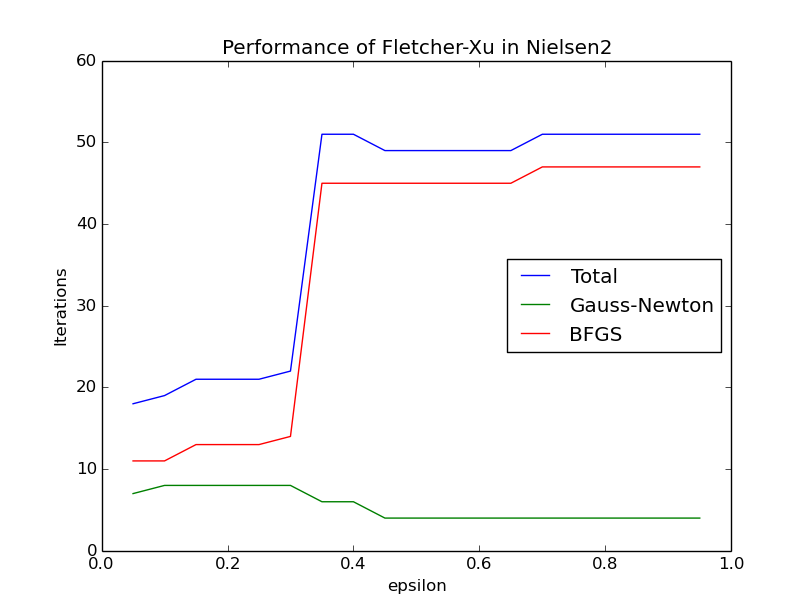
\includegraphics[width=0.65\textwidth]{nielsen2.png}
        \caption{Iterations of Fletcher-Xu in Nielsen2}
        \label{Nielsen2}
\end{figure}
Lastly, the number of iterations for the Trig problem was constantly 27 with 1 Gauss-Newton
and 26 BFGS steps. As this problem has a large residual nearly everywhere, this is not surprising. \par
Summarizing these results one sees that the choice was only significant in Nielsen2. We will later
see  that this problem is the most challenging one for all algorithms. The results for
all other problems are to be expected and are on par with the theoretical properties of
the algorithm. It can be concluded that the recommendation of $\epsilon=0.2$ is an effective choice.
\section{Test Results}
\label{test}
\begin{table}[H]
  \centering
  \begin{tabular}{|l|c|c|c|c|c|}
    \hline
    & Freudenstein & Classical & Nielsen1 &Nielsen2 & Trig  \\ \hline
 MNewton &9&16&6&21&9 \\ \hline
Gauss-Newton &6&5&13&33&x \\ \hline
 appNew &8&9&5&x&8 \\ \hline
 BFGS &17&29&8&40&29 \\ \hline
 MBFGS &10&11&7&54&26 \\ \hline
 Brown-Dennis &8&10&7&x&8 \\ \hline
 DGW &7&6&7&x&17 \\ \hline
 Fletcher-Xu &8&7&7&19&27 \\ \hline
  \end{tabular}
  \caption{Number of Iterations in all 5 Problems}
  \label{tab:iter}
\end{table}
The following Table \ref{tab:iter} shows the number of iterations each method needed to converge.
More details can be found in the appendix, which we will occasionally refer to in this section.
In every table, x denotes a failure of the method. Note that BFGS converged to the strictly local minimum in
Freudenstein's problem, while all others converged to the global one. This behavior is certainly dependent on the line-search parameters, but it is still interesting
to note that MBFGS with the same line-search converged to the global minimum. \par
Let us first compare Brown-Dennis, Fletcher-Xu and DGW. These are the algorithms specifically designed to solve large residual non-linear least squares problems.
All three algorithms performed similarly well in Freudenstein, Classical and Nielsen1. While Fletcher-Xu was still able to converge in Nielsen2, the other two algorithms
failed. This is surprising, especially considering that even Gauss-Newton converged here. But, in the Trig problem, all three algorithms converge and Brown-Dennis even
outperforms Newton's method. This is the only problem where the residual is not just large at the starting point, but also at the solution.  The update strategy
of DGW was slightly better than Brown-Dennis in all but the Trig problem. Maybe the trust-region-switch-model algorithm surrounding their update strategy would
have improved the result here. But, in lights of the results in the Appendix, Brown-Dennis is much more costly than DGW or Fletcher-Xu. This is due to
the fact that every $\nabla^2 r_j$ gets updated individually. \par
It should be noted that Gauss-Newton performs very competitively for the first three if not four problems while being also very cheap to compute.
It fails to converge in the last problem, so it seems to struggle with large residual at the solution, while it can handle large residuals at the starting point.
MNewton and appNewton performed very well throughout, but while the first one requires Hessian constructions, the latter one approximates them with a huge number of
gradient evaluations. This method also failed to converge in Nielsen2, which broke many algorithms.  \par
Both BFGS and MBFGS obviously converged from every point. BFGS's performance was mediocre, while MBFGS was competitive in the first three problems.
In fact, BFGS only beat MBFGS in Nielsen2. This shows that the modification do actually often yield better results in non-linear least squares problems.
When looking at the appendix, one should consider the number of matrix factorizations with precautions: one could implement MBFGS just like BFGS
in a way that the inverse of the Hessian gets approximated. In that case, no matrix factorizations are necessary. Note that the same cannot be said about
Fletcher-Xu, as it also takes Gauss-Steps, which can only approximate the Hessian, but not its inverse. Therefore, one has to use a BFGS update formula
for the Hessian here.\par
It is interesting to note that Fletcher-Xu seems to switch rather efficiently between Gauss-Newton and MBFGS despite its rather simple decision strategy.\par
Overall, the update strategy of Brown-Dennis often works well, especially in the case when the residue of the solution was large. But, on the other hand, it is very costly.
DGW is cheaper, but performed poorly in  the last problem which is very surprising. It seems as if a modified update strategy by itself is not the the answer to
large residual non-linear least squares problems. Fletcher-Xu is very stable paired with decent performance and relatively cheap steps. It performs
better than BFGS and MBFGS and is more stable than Gauss-Newton. Its steps are much cheaper than the steps in appNew and does not require the Hessian like MNewton.
If it could be implemented without matrix factorizations, it would be the absolute clear winner, but even with this one flaw it is my general recommendation.
One could also fix this flaw by transforming it into an iterative method. The BFGS update is of course very well suited for such an approach,
the difficulty lies in handling the Gauss-Newton steps and the steps where the method switches. Nevertheless, such an approach would be feasible and could be implemented memory efficient.
\section{Appendix: Detailed Test Results}
In this appendix, you can find detailled test results. Here, FncEval stands for function evaluations and
JEval stands for evaluations of J(x). These results are analyzed in the section \ref{test}.
\begin{table}[H]
  \centering
  \begin{tabular}{|l|c|c|c|c|c|}
    \hline
  \textbf{Freudenstein} & FncEval &JEval& Matrix-Vector &Matrix-Matrix & Factorizations  \\ \hline
 MNewton &17&9&9&0&8 \\ \hline
Gauss-Newton &13&13&0&8&6 \\ \hline
 appNew &0&29&8&0&8 \\ \hline
 BFGS &45&18&69&68&0 \\ \hline
 MBFGS &21&21&50&32&10 \\ \hline
 Brown-Dennis &0&21&32&33&8 \\ \hline
 DGW &0&8&57&57&7 \\ \hline
 Fletcher-Xu &15&15&15&15&7 \\ \hline
  \end{tabular}
  \caption{Detailed Results Freudenstein}
  \label{tab:Freud}
\end{table}
\begin{table}[H]
  \centering
 \begin{tabular}{|l|c|c|c|c|c|}
    \hline
  \textbf{Classical} & FncEval &JEval& Matrix-Vector &Matrix-Matrix & Factorizations  \\ \hline
  Newton &37&16&16&0&23 \\ \hline
Gauss-Newton &11&11&0&7&5 \\ \hline
 appNew &0&48&9&0&9 \\ \hline
 BFGS &63&30&117&116&0 \\ \hline
 MBFGS &23&23&55&35&11 \\ \hline
 Brown-Dennis &0&121&200&201&8 \\ \hline
 DGW &0&7&49&49&6 \\ \hline
 Fletcher-Xu &13&13&5&10&6 \\ \hline
  \end{tabular}
  \caption{Detailed Results Classical}
  \label{tab:Class}
\end{table}
\begin{table}[H]
  \centering
 \begin{tabular}{|l|c|c|c|c|c|}
    \hline
  \textbf{Nielsen1} & FncEval &JEval& Matrix-Vector &Matrix-Matrix & Factorizations  \\ \hline
  MNewton &11&6&6&0&5 \\ \hline
Gauss-Newton &27&27&0&15&13 \\ \hline
 appNew &0&36&5&0&5 \\ \hline
 BFGS &18&9&33&32&0 \\ \hline
 MBFGS &15&15&35&23&7 \\ \hline
 Brown-Dennis &0&91&140&141&7 \\ \hline
 DGW &0&8&57&57&7 \\ \hline
 Fletcher-Xu &13&13&15&14&6 \\ \hline
  \end{tabular}
  \caption{Detailed Results Nielsen1}
  \label{tab:Nielsen1}
\end{table}
\begin{table}[H]
  \centering
 \begin{tabular}{|l|c|c|c|c|c|}
    \hline
  \textbf{Nielsen2} & FncEval &JEval& Matrix-Vector &Matrix-Matrix & Factorizations  \\ \hline
  MNewton &44&21&21&0&97 \\ \hline
Gauss-Newton &69&67&0&35&33 \\ \hline
 appNew &x&x&x&x&x \\ \hline
 BFGS &108&41&161&160&0 \\ \hline
 MBFGS &109&109&270&164&54 \\ \hline
 Brown-Dennis &x&x&x&x&x \\ \hline
 DGW &x&x&x&x&x \\ \hline
 Fletcher-Xu &47&37&55&45&18 \\ \hline
  \end{tabular}
  \caption{Detailed Results Nielsen2}
  \label{tab:Nielsen2}
\end{table}
\begin{table}[H]
  \centering
 \begin{tabular}{|l|c|c|c|c|c|}
    \hline
  \textbf{Trig} & FncEval &JEval& Matrix-Vector &Matrix-Matrix & Factorizations  \\ \hline
  MNewton &17&9&9&0&8 \\ \hline
Gauss-Newton &x&x&x&x&x \\ \hline
 appNew &0&65&8&0&8 \\ \hline
 BFGS &117&30&130&116&0 \\ \hline
 MBFGS &84&53&130&80&26 \\ \hline
 Brown-Dennis &0&201&320&321&8 \\ \hline
 DGW &0&18&137&137&17 \\ \hline
 Fletcher-Xu &85&53&130&8&27 \\ \hline
  \end{tabular}
  \caption{Detailed Results Trig}
  \label{tab:Trig}
\end{table}
\nocite{Nocedal2004}\nocite{Gille1978}\nocite{Fletcher1986}
\bibliographystyle{alpha}
\bibliography{library}
\end{document}